\documentclass[conference]{IEEEtran}
\IEEEoverridecommandlockouts                              
%\overrideIEEEmargins
\usepackage[utf8]{inputenc}
\usepackage[T1]{fontenc}
\usepackage{hyperref}
\usepackage{xcolor}
\usepackage{graphicx}
\usepackage{amsmath}
\graphicspath{{./images/}}

\begin{document}
\title{Basics of data structure needed for state-space search tasks and use of random numbers required for MDP and RL}
% author names and affiliations
\author{\IEEEauthorblockN{Mukesh Vaishnav}
\IEEEauthorblockA{202051196}
\and
\IEEEauthorblockN{Kaushik Rathva}
\IEEEauthorblockA{202051156}
\and
\IEEEauthorblockN{Patel Jaykumar}
\IEEEauthorblockA{202051136}
\and
\IEEEauthorblockN{Sontakke Ajinkya}
\IEEEauthorblockA{202051179}
}
% make the title area
\maketitle
\setlength{\parindent}{20pt}
\noindent Github link: \href{https://github.com/JARVIS-codebase/LAB-8}{LAB-8} \\ \\ 
\indent \begin{abstract}
Understanding MENACE by Michie and examining its application are our goals. to draw attention to and clarify the code's key components.
\end{abstract}
\IEEEpeerreviewmaketitle

\section{Introduction}
Tic-tac-toe is played using the machine learning algorithm Menace. Matchbox Educable Noughts And Crosses Engine is referred to as Menace. The method is built upon a set of matchboxes that contain game board configurations and Menace's prior moves for each arrangement. Menace learns to change the probabilities of performing particular moves according on the results of the games by playing a lot of games against random opponents. The probabilities are kept in each matchbox as weights assigned to each move. When playing a game, Menace consults its matchboxes to determine the current board layout, selects the move with the highest weight, and then modifies the weight of that move after it has been executed.
\section{Problem Statement} 
Read the reference on MENACE by Michie and check for its implementations.  Pick the one that you like the most and go through the code carefully.  Highlight the parts that you feel are crucial.  If possible, try to code the MENACE in any programming language of your liking.
\\
\\
\\
\\
\section{Code Summary} 
The code to play tic tac toe contains a description of the Menace algorithm. The Menace player engages in a series of games against an undetermined foe in an effort to discover the most effective tactics. The algorithm consists of these three key tasks:

The $play\_game()$ function initiates a Tic Tac Toe match between the Menace player and a chosen opponent.

The $choose\_move\_index()$ function chooses an index from a list of move weights, using a weighted random choice.\\
\\

Tic Tac Toe games are used to train the Menace player in the $train\_menace()$ function. A Menace player, a Tic Tac Toe board, and a flag indicating whether to print the game board while the game is in progress are required by the $play\_game()$ function. A dictionary containing lists of move weights as values serves as the Menace player and keys that indicate the board's current status. The function rotates between the Menace player and the random player up until a winner is established or the game concludes in a draw. Every turn, the function selects the move with the highest weight and adjusts the weights for that move in the Menace player dictionary.

The $choose\_move\_index()$ function uses a weighted random selection to choose an index from a list of move weights. The weight of a move affects how likely it is to be chosen. In order to teach the Menace player, the $train\_menace()$ function engages in a number of Tic Tac Toe games. The $play\_game()$ function is used by the function to play the game and initialise a fresh board for each game. The function adds the weights for the moves made throughout the game to the Menace player dictionary after each game. The trained Menace player dictionary is returned by the function.

\section{Results}
After playing many hundred games of tic-tac-toe in the physical implementation, MENACE was able to master the game to a level that was comparable to human players. In the simulation, MENACE was able to master the game of tic-tac-toe after playing several thousand games against a random opponent, and after playing tens of thousands of games, MENACE was able to master more difficult forms of the game.\\

To answer the question, "What grade would a student get in PH100?" we generated conditional probability tables of all the nodes with the criterion that a student receives DD in EC100, CC in IT101, and CD in MA101. The results of this study indicated that there is a 92 percent chance that the student will receive a CD in PH100.

\section{Outputs}
$$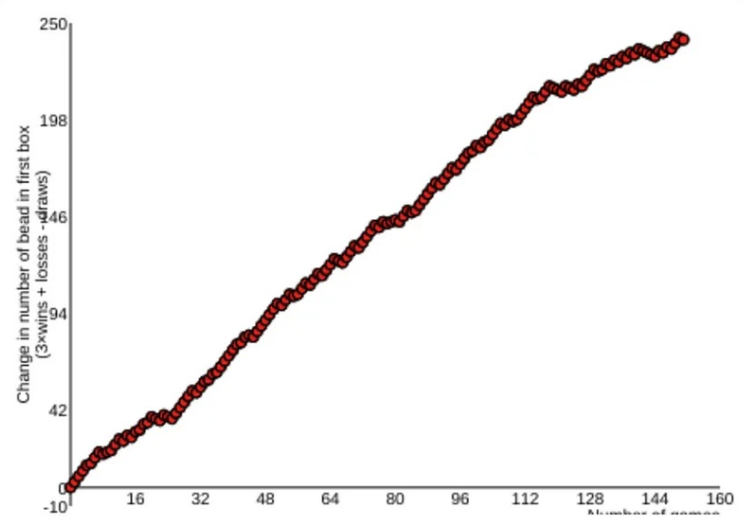
\includegraphics[scale=0.5]{images/8.2.png}$$
$Fig. \; MENACE \; score \; when \; played \; against \; a \; random \; \\opponent$
$$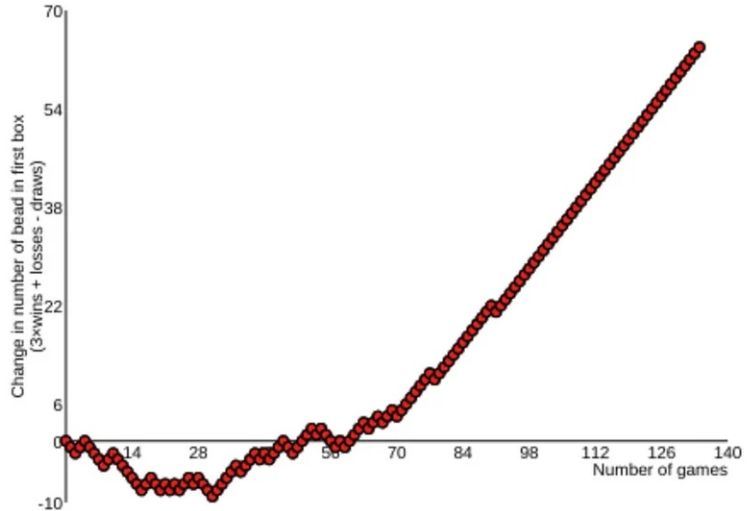
\includegraphics[scale=0.5]{images/8.1.png}$$
$Fig. \; MENACE \; score \; when \;  played \; against \; a \; perfect-playing \; opponent$

\section{CONCLUSION}
Menace initially loses while learning, but eventually begins to win while playing against a random opponent. The MENACE experiment showed how a straightforward reinforcement learning system may gradually enhance its gaming prowess through trial and error. MENACE learnt which moves were more likely to lead to a win based on the prizes and penalties it got after each game using matchboxes packed with coloured beads to represent moves. The experiment also demonstrated how crucial it is to eliminate redundant states in order to minimise the quantity of matchboxes required.
\begin{thebibliography}{}
\bibitem{}
Donald Michie\emph{Experiments on the mechanization of game-learning} \href{http://people.csail.mit.edu/brooks/idocs/matchbox.pdf}{http://people.csail.mit.edu/brooks/idocs/matchbox.pdf}
\bibitem{}
Tanmay Ambadkar (2021) Artificial Intelligence Course. \href{https://github.com/TanmayAmbadkar/CS302-AI/tree/master/Lab8}{https://github.com/TanmayAmbadkar/CS302-AI/tree/master/Lab8}(2021).
\end{thebibliography}
\end{document}


